% THIS TEMPLATE IS A WORK IN PROGRESS

\documentclass[polish, a4paper]{article}
\usepackage[a4paper,left=3cm,right=3cm,top=3cm,bottom=1.5cm]{geometry}
\usepackage[T1]{fontenc}
\usepackage[polish]{babel}
\usepackage[utf8]{inputenc}
\usepackage{hyperref}
\usepackage{fancyhdr}
\usepackage{float}
\usepackage{graphicx}
\usepackage{titling}
\usepackage{wasysym}
\usepackage{caption}
\usepackage{pgfplots}
\usepackage{pgfplotstable}
\usepackage{filecontents}
\usepackage{csvsimple}
\usepackage{textcomp}
\usepackage{gensymb}
\usepackage{etoolbox}
%\usepackage{siunitx}
\graphicspath{ {./} }
\pagestyle{fancy}

\setlength{\droptitle}{-1in}

%\lhead{\includegraphics[width=0.2\textwidth]{nyush-logo.pdf}}

  \lhead{Maciej Kaszkowiak}
  \chead{Warstwa transportowa}
  \rhead{
  151856}


%%%% PROJECT TITLE
\title{Routing statyczny Cisco\\
        \Large \emph{Sprawozdanie nr 6 z przedmiotu Sieci Komputerowe}}

%%%% NAMES OF ALL THE STUDENTS INVOLVED (first-name last-name)
\author{Maciej Kaszkowiak, 151856, zadania wykonane 3 czerwca 2023}

\date{\vspace{-5ex}} %NO DATE


\begin{document}

\maketitle
%\thispagestyle{titlepage}

\tableofcontents

\newpage

\section{Przy pomocy programu netstat zbadaj, na jakich portach
uruchamiane są serwery:}

\begin{itemize}
\item{HTTP - 80}
\item{HTTPS - 443}
\item{FTP - 21}
\item{telnet - 23}
\item{DNS - 53}
\end{itemize}

Oraz kilka dodatkowych:
\begin{itemize}
\item{ssh - 22}
\item{PostgreSQL - 5432}
\item{Redis - 6379}
\item{MongoDB - 27019}
\end{itemize}

Zauważyłem również, że Google Chrome jako \emph{klient} ma losowo przydzielane porty. 

\section{Zadanie 3}
\subsection{Przeprowadzić analizę komunikacji (Wireshark) na poziomie warstwy transportowej
podczas przykładowej transmisji w systemie WWW.}

Załadowałem plik http.cap do programu Wireshark.

\subsection{
Określić adresy IPv4 i numery portów (klienta i serwera) używanych podczas transmisji.
}

W przypadku połączenia o download.html, IPv4 serwera to 65.208.228.223, zaś IP klienta to 145.254.160.237. Port serwera to 80 (HTTP), a port klienta (przeglądarki) to 3372. Możemy zauważyć również połączenie na porcie 3371 - jest to drugie zapytanie ujęte w pliku http.cap, odpytujące o reklamy.  

\begin{figure}[H]
\centering
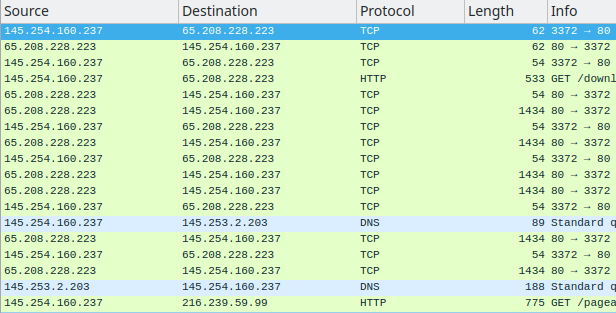
\includegraphics[width=\textwidth]{internet.png}
\caption{Adresy oraz nr portów}
\end{figure}

\subsection{
Przeprowadzić analizę segmentów TCP przesyłanych w trakcie nawiązywania połączenia
między klientem a serwerem HTTP. Określić dla każdego segmentu:
}

\begin{itemize}
\item{kierunek transmisji}
\item{numery portów (źródłowego, docelowego)}
\item{znaczniki}
\item{wartość pola sequence number}
\item{wartość pola acknowledge number}
\item{wartość pola window size}
\item{wartości opcji}
\end{itemize}

\begin{figure}[H]
\centering
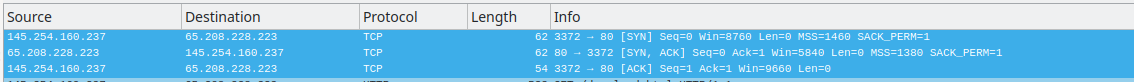
\includegraphics[width=\textwidth]{polaczenie.png}
\caption{Nawiązywanie połączenia pomiędzy klientem a serwerem HTTP}
\end{figure}

Na zrzucie ekranu możemy zaobserwować TCP handshake w postaci trzech pakietów (SYN, SYN ACK, ACK). Pakiet SYN trafia od klienta do serwera, SYN ACK od serwera do klienta, zaś ACK ponownie od klienta do serwera. Po wymianie pakietów transmisja zostaje nawiązana.

Poniżej zamieściłem informacje z Wiresharka. Przykładowo, pierwszy pakiet informuje o przesyłaniu danych z adresu 145.254.160.237:3372 na adres 65.208.228.223:80, ze znacznikiem SYN, z polem sequence number o wartości 0, bez wartości acknowledge number, z polem window size równym 8760, z opcjami MSS = 1460  (maksymalny rozmiar segmentu) oraz SACK PERM = 1.

\begin{figure}[H]
\begin{verbatim}
145.254.160.237	65.208.228.223	TCP	62	3372 → 80 [SYN] Seq=0 
  Win=8760 Len=0 MSS=1460 SACK_PERM=1
  
65.208.228.223	145.254.160.237	TCP	62	80 → 3372 [SYN, ACK] Seq=0 Ack=1 
  Win=5840 Len=0 MSS=1380 SACK_PERM=1
  
145.254.160.237	65.208.228.223	TCP	54	3372 → 80 [ACK] Seq=1 Ack=1 
  Win=9660 Len=0
\end{verbatim}
\caption{Przedruk z Wiresharka}
\end{figure}

Poniżej załączam przedruk z RFC odnośnie opcji SACK\_PERM:

\begin{figure}[H]
\begin{verbatim}
2.  Sack-Permitted Option
This two-byte option may be sent in a SYN by a TCP that has been
   extended to receive (and presumably process) the SACK option once the
   connection has opened.  It MUST NOT be sent on non-SYN segments.

\end{verbatim}
\caption{RFC 2018: TCP Selective Acknowledgment Options}
\end{figure}


\subsection{
Przeprowadzić analizę segmentów TCP przesyłanych w trakcie przesyłania zawartości
strony download.html między serwerem HTTP a klientem. Określić dla każdego segmentu:
}
\begin{itemize}
\item{kierunek transmisji}
\item{numery portów (źródłowego, docelowego)}
\item{znaczniki}
\item{wartość pola sequence number}
\item{wartość pola acknowledgement number}
\item{wielkość pola danych.}
\end{itemize}

\begin{figure}[H]
\centering
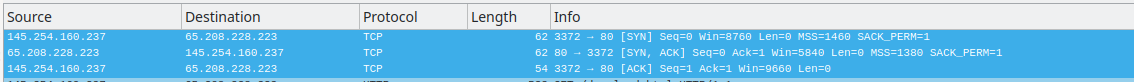
\includegraphics[width=\textwidth]{polaczenie.png}
\caption{Połączenie HTTP pomiędzy klientem a serwerem HTTP}
\end{figure}

\begin{figure}[H]
\centering
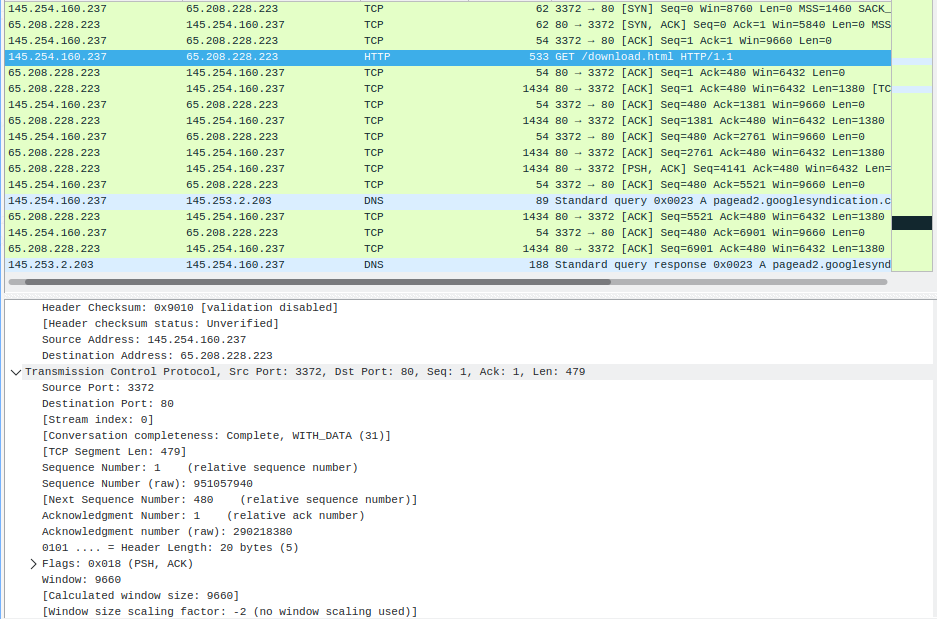
\includegraphics[width=\textwidth]{HTTP.png}
\caption{Żądanie HTTP}
\end{figure}

Na zrzutach ekranu możemy zaobserwować, że początkowo przesyłany jest pakiet z flagami PSH/ACK z żądaniem GET o pobranie pliku. W odpowiedzi serwer wysyła pakiety z danymi oraz flagą ACK. Klient zaś potwierdza każdy pakiet odpowiadając pakietem ACK bez danych. Wartości sequence number rosną wraz z przesyłem danych, a acknowledgement number odpowiada odpowiednim polom sequence number. Adresy IP oraz numery portów pozostają bez zmian. IPv4 serwera WWW to 65.208.228.223, zaś IP klienta (przeglądarki) to 145.254.160.237. Port serwera to 80, a port klienta to 3372.

\subsection{
Przeprowadzić analizę segmentów TCP przesyłanych w trakcie rozłączania. Określić dla
każdego segmentu:
}
\begin{itemize}
\item{kierunek transmisji}
\item{numery portów (źródłowego, docelowego)}
\item{znaczniki}
\item{wartość pola sequence number}
\item{wartość pola acknowledge number.}
\end{itemize}

\begin{figure}[H]
\centering
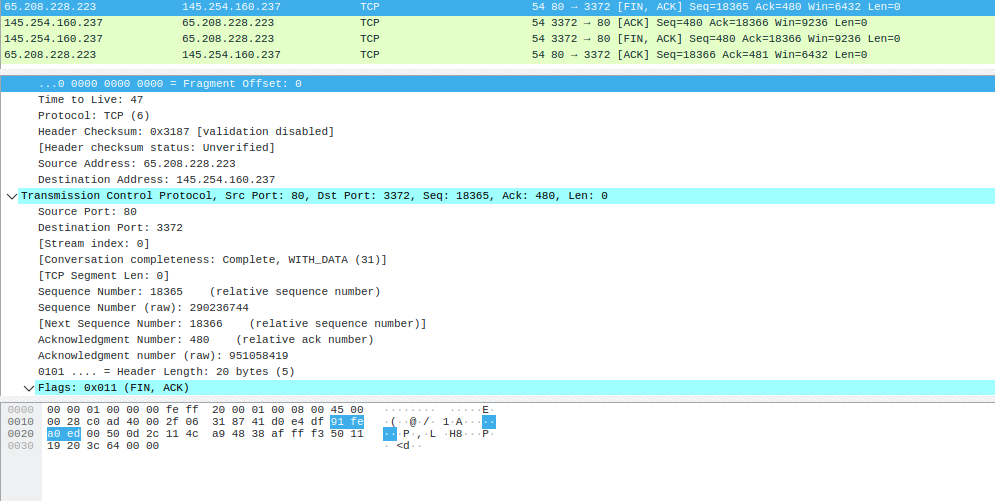
\includegraphics[width=\textwidth]{koniec.png}
\caption{Segmenty TCP}
\end{figure}

Możemy zaobserwować, że koniec transmisji odbywa się zgodnie z następującym schematem: Klient przesyła do serwera pakiet FIN ACK, na co serwer odpowiada pakietem ACK. Następnie serwer również potwierdza zakończenie transmisji, przesyłając pakiet FIN ACK, na co klient odpowiada pakietem ACK. Adresy IP oraz numery portów pozostają bez zmian. IPv4 serwera WWW to 65.208.228.223, zaś IP klienta (przeglądarki) to 145.254.160.237. Port serwera to 80, a port klienta to 3372. 


\end{document}